% =============================================================================
% §3 SkillCorpus (~1.5 pages)
% =============================================================================
\section{SkillCorpus}
\label{sec:corpus}

% FIG 1 (fig:pipeline) declared at the top of §3 (method) so the full-width [t]
% float lands on the method page. AAAI bans stfloats/dblfloatfix, so placement
% is controlled by the declaration point.
\begin{figure*}[t]
\centering
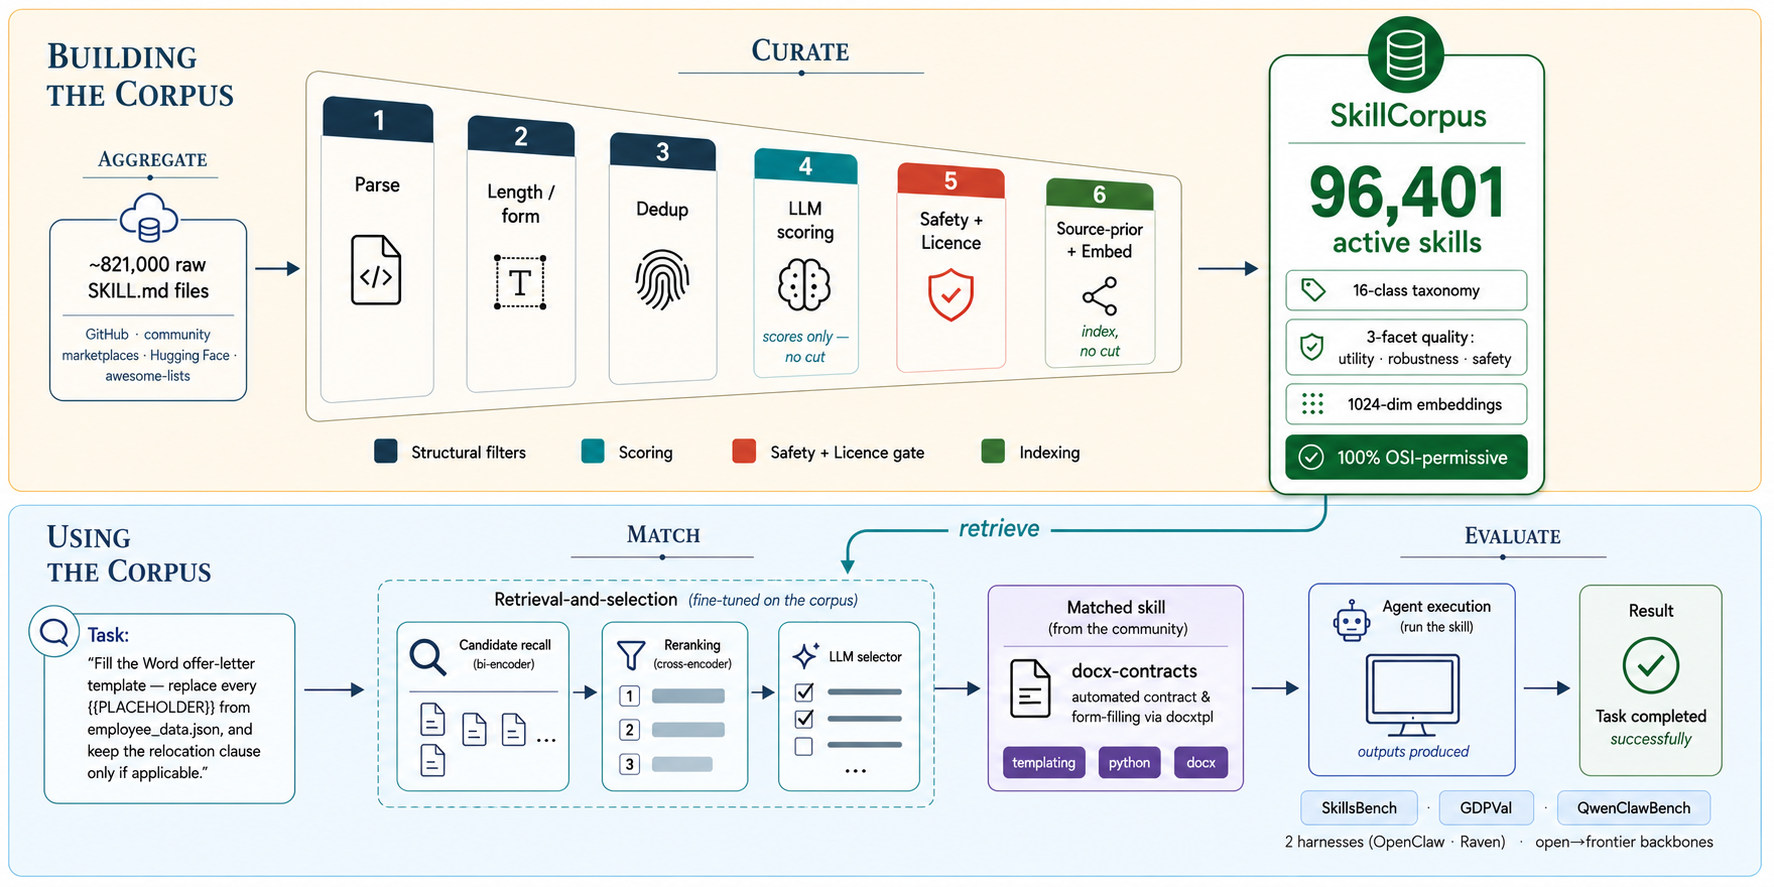
\includegraphics[width=\textwidth]{figures/fig_pipeline_v10.png}
\caption{The SkillCorpus framework.  Building the corpus (top), we
aggregate community \texttt{SKILL.md} files from public source
channels and curate them through a six-stage funnel into a
$96{,}401$-skill corpus organised by a 16-class taxonomy and three
quality facets.  Using the corpus (bottom), a fine-tuned
retrieval-and-selection stack matches skills to an incoming task and
an agent runs the selected skill end-to-end.  The worked example
traces one real task from request to result, and we evaluate this
pipeline across three real-world benchmarks, two harnesses, and
open-to-frontier backbones.}
\label{fig:pipeline}
\end{figure*}

% \paragraph{Skill specification.}
% We adopt the \texttt{SKILL.md} convention of
% \citet{AnthropicSkillCreator2025} verbatim.  Each skill is a
% self-contained directory whose \texttt{SKILL.md} file carries
% required YAML frontmatter (\texttt{name}, \texttt{description})
% plus a Markdown procedural body, optionally bundled with
% executable resources.  The ingest pipeline below admits only
% files conforming to this contract, matching the loading
% convention used by the agent harnesses in
% \S\ref{sec:experiments}.

\ifarxiv
SkillCorpus is a single end-to-end framework that turns the open \texttt{SKILL.md} ecosystem into a curated, deployable corpus and measures its effect on real-world agent tasks. As shown in Figure~1, it runs in four stages: aggregation and curation of the ecosystem into a corpus (\S3.1–\S3.3), matching of task-relevant skills via a fine-tuned retrieval-and-selection stack (\S3.4), and end-to-end evaluation on real-world agent tasks (\S\ref{sec:experiments}).
\else
As shown in Figure~1, SkillCorpus runs in four stages: aggregation and curation of the ecosystem into a corpus (\S3.1–\S3.3), matching of task-relevant skills via a fine-tuned retrieval-and-selection stack (\S3.4), and end-to-end evaluation on real-world agent tasks (\S\ref{sec:experiments}).
\fi

% --------------------------------------------------------- 3.1 pipeline ------
\subsection{Multi-source aggregation and the curation pipeline}
\label{sec:pipeline}

The corpus's value is its coverage, spanning the whole public
ecosystem rather than a single channel.
The crawl is driven by a single machine-readable source
registry of $62$ sources, detailed in
Appendix~\ref{app:crawl-sources}.  The registry spans five
ingestion mechanisms, from directly cloned repositories and
awesome-list scrapes to marketplace index APIs, sitemap crawls,
and JSON catalogs, and every mechanism feeds one shared discovery
entry point.  Our crawl gathers $\sim$$821{,}000$ raw \texttt{SKILL.md} files.
After source selection and repository-level de-duplication,
$25{,}159$ GitHub repositories feed the six-stage pipeline, which
curates them into the released active set.

Figure~\ref{fig:pipeline} visualises the pipeline.
% Stages~1--2 apply structural filters on the
% \texttt{SKILL.md} contract (parse and length/form).  
Each skill follows the \texttt{SKILL.md} convention of \citet{AnthropicSkillCreator2025} — a Markdown body with optional executable resources; Stages 1–2 apply structural filters on this contract (parse and length/form).
Stage~3 deduplicates.  Stage~4 runs the LLM judge that emits the
3-facet quality score and 19 safety/quality flags.  Stage~5
applies the safety hard-gate plus
Open Source Initiative (OSI)-permissive licence filter
(Table~\ref{tab:license-filter}).  Stage~6 attaches source-prior
shrinkage, the 1024-dim retrieval embedding, and index entries.
Parse and deduplication dominate the funnel, while the remaining
filters contribute a few percent.

\paragraph{Two-tier deduplication (stage 3).}
Deduplication is the funnel's steepest reduction
($283{,}844 \to 101{,}111$, $-64\%$), in two tiers.  An exact tier
collapses $169{,}465$ content- and name-fingerprint duplicates,
$59.7\%$ of the stage input, which reflects how
heavily the ecosystem replicates the same artifacts across
repositories.  A semantic tier embeds each survivor (1024-dim)
and flags pairs above cosine $0.90$, and pairs above $0.995$
merge automatically.  The $66{,}751$ borderline pairs are adjudicated
by an LLM judge, which confirms $25.4\%$ of pairs and collapses
$13{,}268$ near-duplicate skills.  The resulting low-overlap
distribution also lets the retrieval stack train on the corpus
itself.

% --------------------------------------------------------- 3.2 quality -------
\subsection{Three-facet quality framework}
\label{sec:quality}

\ifarxiv
We decompose skill quality into three
facets, each capturing a distinct concern, rather than
collapsing them into a single composite or a flat
multi-dimensional list.
\else
We decompose skill quality into three facets, each capturing a
distinct concern rather than a single composite.
\fi
These facets serve curation and
retrieval ranking, with the safety facet additionally serving the
release gate, as characterised in \S\ref{sec:claim-a}.

\paragraph{Three facets.}
The utility facet scores the description alone, asking whether the
task class is well-scoped with clear triggers and applicability
conditions.  The robustness facet scores the body content and its
consistency with the description's promise.  A body that is
internally coherent but silently delivers something narrower than
promised is penalised here.  The safety facet captures harm and risk along
categories such as prompt injection, command injection,
credential leakage, and unsafe execution.  By design, the utility and robustness facets are scored
independently.  Description-level issues only affect utility, and
body-level issues only affect robustness.

\paragraph{Flag taxonomy.}
The 19-flag vocabulary is partitioned across the three facets ($2$
utility-bound, $6$ robustness-bound, $11$ safety-bound), with the
full list in Appendix~\ref{app:flags}.  Each flag, when fired, constrains
its assigned facet's score.  Five flags act as hard gates:
\texttt{prompt\_injection}, \texttt{cmd\_injection},
\texttt{unsafe\_exec}, \texttt{auth\_bypass}, and
\texttt{csam\_risk}.  Firing any one of these forces the quality
score to zero and excludes the skill from the released
\texttt{active} set.  The remaining fourteen flags act as soft signals.  When such a
flag fires, the LLM judge caps the corresponding facet score.
A fired \texttt{placeholder} flag, for example, holds robustness
at $\leq 4$.  No additional numeric deduction is applied, so the same
observation is not double-counted.

\paragraph{Facet separation.}
The three facets are not redundant.  The safety facet is markedly
more independent from the two craftsmanship facets
($r(u,s){=}0.15$, $r(r,s){=}0.30$) than those are from each other
($r(u,r){=}0.59$), matching the design, since $u$ and $r$ both
track artifact craftsmanship while $s$ targets an orthogonal harm
axis on which a well-crafted skill can still be unsafe.  We read
these contrasts qualitatively and do not claim construct-validity
orthogonality.  Rigorous validation would require independent human
gold annotation \citep{SkillNet2026}.  The off-diagonal-mass
analysis, the per-pair figure, and the score-bucket distribution
are given in Appendix~\ref{app:quality-detail}.

\paragraph{Score formula.}
Following the LLM-as-judge paradigm \citep{Zheng2023LLMJudge},
the judge outputs three integer subscores $u, r, s$ on
$\{0, \ldots, 10\}$, normalised to $[0, 1]$.  These combine into
$\mathtt{content\_q} = 0.50\,u + 0.35\,r + 0.15\,s$, attenuated by
a factor $0.5 + 0.5\,(s{-}0.3)/0.4$ when the safety subscore is
marginal ($s \in [0.3, 0.7]$).  The final per-skill score, or composite quality score, shrinks
content quality toward a per-source prior
(Appendix~\ref{app:source-prior}):
\[
\mathtt{score} = 0.85\,\mathtt{content\_q} + 0.15\,\mathtt{prior}_{\mathrm{src}} + b,
\]
where $b$ is a small structural bonus
($+0.05$ for skills shipping \texttt{scripts/},
$+0.02$ for \texttt{references/}), and the result is clipped to
$[0, 1]$.

% --------------------------------------------------------- 3.3 classify -----
\subsection{Classification, filtering, and release}
\label{sec:classify}

\paragraph{Taxonomy.}
We adopt a single-label, 16-class taxonomy designed to cover the
observed distribution of community skills while remaining
decision-tree classifiable from \texttt{name},
\texttt{description}, and a short body excerpt.  The classifier
prompt enforces six conflict-resolution rules, the most
consequential being the \textsc{AI-ML} rule that a skill is
labelled \textsc{AI-ML} only when its primary deliverable is an AI
system (persona, agent, or model), not merely when it uses an LLM
internally.  The full rule set is released with the classifier
prompt.

\paragraph{Distribution.}
The class distribution on the active release set is summarised in
Figure~\ref{fig:class-dist}.  The corpus is software- and
data-leaning.  \textsc{Dev}, \textsc{Data}, \textsc{Writing}, and
\textsc{DevOps-Infra} together account for over half of active
skills.  The catch-all \textsc{Other} class is small ($2.01\%$),
indicating that the taxonomy covers the observed distribution well.
Every active skill carries exactly one of the sixteen
classes.

\begin{figure}[!ht]
\centering
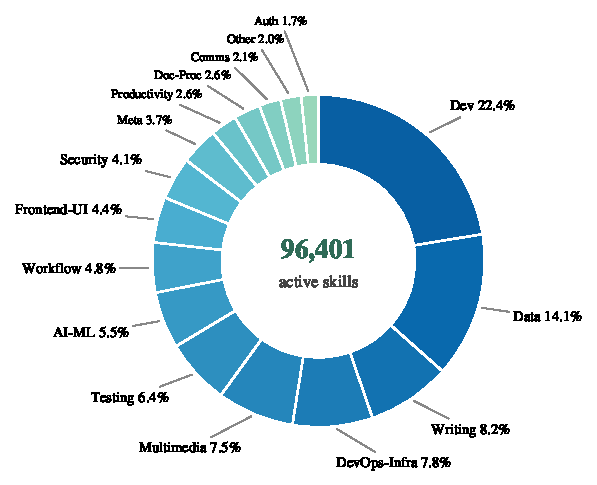
\includegraphics[width=0.96\columnwidth]{figures/fig_class_pie.pdf}
\caption{16-class distribution on the active release set
($N{=}96{,}401$, shares in \%, sorted clockwise).}
\label{fig:class-dist}
\end{figure}

\paragraph{Safety and licence filters (stage 5).}
The two filters run in sequence on the
$\sim$$101$K skills surviving stages 1--4.  A safety hard-gate
removes $915$ skills triggering any of three
conditions: a pre-judge \texttt{blocked.malware} regex match
(Appendix~\ref{app:fp-audit}),
firing of any of the five LLM-judged hard-gate flags defined in
\S\ref{sec:quality}, or an LLM safety subscore below~$3$.  A
licence filter then enriches each source repository's
\texttt{spdx\_id} via the GitHub API and admits only skills
carrying an OSI-approved permissive licence
(Table~\ref{tab:license}), excluding a further $3{,}795$ skills
whose source repositories lack a usable permissive licence
(per-reason counts in Table~\ref{tab:license-filter}).  Every
skill in the resulting $96{,}401$-skill active set is therefore
commercially redistributable under its source repository's
declared licence.

\paragraph{Release.}
The corpus is released as a single artifact comprising the
metadata SQLite database, the per-stage
ingest report of raw counts at each pipeline stage, the precomputed
3-facet quality cache, the 1024-dim retrieval embeddings, and
the retrieval-and-selection stack
used in our experiments and released as engineering tooling.  All
curation source code will be released under a permissive licence
upon acceptance.

% --------------------------------------------------------- 3.4 retrieval ----
\subsection{Retrieval and selection stack}
\label{sec:retrieval}

The corpus is released together with a fine-tuned
retrieval-and-selection stack so the artifact ships ready to use
rather than requiring a retrieval stack to be built.  We use ``deployable'' in this packaging sense, not as a
production-validation claim.  The stack follows the standard
retrieve-then-rerank pattern of retrieval-augmented generation
\citep{Lewis2020RAG}, with three operational stages: candidate
recall, rerank, and final selection by an LLM gate.

\paragraph{Recall and rerank.}
Candidate recall uses an embedding model fine-tuned from
Qwen3-Emb-0.6B.  A scoring model fine-tuned from Qwen3-Rank-0.6B
then reranks the top candidates.  Both models are trained on
the strictly deduplicated active set.  The low-overlap data
distribution is intended to give a cleaner contrastive learning
signal by preventing functionally identical near-duplicates from
being sampled as hard negatives, which could otherwise produce
false-negative collisions during contrastive fine-tuning.  We
adopt this as a training-design rationale rather than an isolated
ablation.  Recall and rerank operate over a
$3{,}000$-character retrieval field distilled from each skill
body, avoiding length-induced truncation noise.

\paragraph{LLM selector (gate).}
Reranked top-$k$ candidates can still include topically
irrelevant items, and brief summaries are insufficient for an
agent to judge tool fit at execution time.  We therefore insert
an LLM selector that, given the task query and the full skill
body of each reranked candidate, returns $0$--$2$ precise tools
for injection into the agent prompt.  This trades one additional
LLM call for the reliability of full-body inspection while
keeping the injected context within strict per-task budgets.

\paragraph{Query rewriter (optional).}
An optional LLM-based query rewriter normalises domain-specific
jargon in the task description to vocabulary that better matches
the corpus's skill descriptions, and is permitted to short-circuit
(no skills required) when the task is clearly outside the
corpus's scope.

We evaluate this stack both as part of the end-to-end pipeline,
where it drives the main-grid pass-rate gains, and as a
standalone retrieval system on Hit@1 / Recall@10 against
published baselines.
